\documentclass[12pt,a4paper]{report}
\usepackage[utf8]{inputenc}
\usepackage[T1]{fontenc}
\usepackage{graphicx}
\usepackage{hyperref}
\usepackage{geometry}
\usepackage{booktabs}
\usepackage{xcolor}
\usepackage{listings}
\usepackage{amsmath}
\usepackage{amssymb}
\usepackage{float}
\usepackage{caption}
\usepackage{subcaption}
\usepackage{setspace}
\usepackage{titlesec}
\usepackage{fancyhdr}
\usepackage{mdframed}
\usepackage{tikz}
\usetikzlibrary{shapes.geometric, arrows, positioning, shadows, backgrounds}

% TikZ Styles
\tikzstyle{sensor} = [rectangle, rounded corners, minimum width=2.5cm, minimum height=1cm, text centered, draw=blue!50, fill=blue!5, thick]
\tikzstyle{process} = [rectangle, minimum width=3cm, minimum height=1cm, text centered, draw=orange!70, fill=orange!10, thick]
\tikzstyle{modality} = [diamond, minimum width=2cm, minimum height=1cm, text centered, draw=cyan!70, fill=cyan!5, inner sep=0pt, font=\footnotesize]
\tikzstyle{decision} = [rectangle, rounded corners, minimum width=3cm, minimum height=1cm, text centered, draw=red!70, fill=red!10, thick]
\tikzstyle{arrow} = [thick,->,>=stealth, color=gray!80]

\geometry{margin=1in, top=1.2in, bottom=1.2in}
\onehalfspacing

\hypersetup{
    colorlinks=true,
    linkcolor=blue!70!black,
    urlcolor=cyan!60!black,
    citecolor=green!50!black
}

% Code listing style
\definecolor{codegray}{rgb}{0.95,0.95,0.95}
\definecolor{codegreen}{rgb}{0,0.5,0}
\definecolor{codepurple}{rgb}{0.55,0,0.55}
\definecolor{codeblue}{rgb}{0.1,0.1,0.8}

\lstdefinestyle{pythonstyle}{
    backgroundcolor=\color{codegray},
    commentstyle=\color{codegreen}\itshape,
    keywordstyle=\color{codeblue}\bfseries,
    numberstyle=\tiny\color{gray},
    stringstyle=\color{codepurple},
    basicstyle=\ttfamily\footnotesize,
    breakatwhitespace=false,
    breaklines=true,
    captionpos=b,
    keepspaces=true,
    numbers=left,
    numbersep=5pt,
    showspaces=false,
    showstringspaces=false,
    showtabs=false,
    tabsize=4,
    language=Python,
    frame=single,
    rulecolor=\color{gray!40}
}

% Header/Footer
\pagestyle{fancy}
\fancyhf{}
\rhead{Sentinel KYC Research}
\lhead{Fahad Nafees}
\cfoot{\thepage}

% Custom box for research notes
\newmdenv[
  topline=true,
  bottomline=true,
  rightline=false,
  leftline=true,
  linewidth=3pt,
  linecolor=blue!40,
  backgroundcolor=blue!5,
  innerleftmargin=10pt,
  innerrightmargin=10pt
]{researchbox}

%------------------------------------------------------------------
%   TITLE PAGE
%------------------------------------------------------------------
\begin{document}

\begin{titlepage}
    \centering
    \vspace*{2cm}
    {\huge\bfseries Sentinel KYC:\par}
    \vspace{0.5cm}
    {\Large\bfseries A Multi-Modal Framework for Liveness Detection and Anti-Spoofing Research\par}
    \vspace{2cm}
    {\Large Fahad Nafees\par}
    {\large\itshape Independent Research Project\par}
    \vspace{1cm}
    \vspace{1.5cm}
    \rule{\linewidth}{0.5pt}
    \vspace{0.5cm}
    {\large \today\par}
    \vspace{2cm}
    \begin{abstract}
    The \textbf{Sentinel KYC} system is a research-grade, multi-modal biometric liveness detection framework implemented in Python using OpenCV, MediaPipe, SciPy, and Streamlit. The system is designed to investigate the technical feasibility of detecting identity spoofing attacks in real time through a combination of geometric analysis, physiological signal extraction, frequency domain analysis, temporal pattern recognition, and 3D depth estimation. This document provides a comprehensive technical description of each modality implemented, including the specific algorithms, mathematical formulations, code logic, and experimental thresholds used in the research prototype. The system also incorporates a weighted Decision Engine that fuses all modality signals into a single confidence-scored liveness verdict.
    \end{abstract}
    \vfill
\end{titlepage}

\tableofcontents
\listoffigures
\newpage

%------------------------------------------------------------------
%   CHAPTER 1: INTRODUCTION
%------------------------------------------------------------------
\chapter{Introduction}

\section{Motivation}
Know Your Customer (KYC) systems are the first line of defence in digital identity verification. As remote onboarding becomes the norm in banking, fintech, and government services, the risk of presentation attacks---also called spoofing---has grown significantly. An attacker may present a high-resolution printed photograph, a looping video played on a tablet, a 3D-printed silicone mask, or even a real-time digitally injected stream using deepfake software. Classical static biometric checks (comparing a selfie to a passport photo) are insufficient to defeat these threats.

\section{Objectives}
This research project explores the following hypothesis: \textit{A combination of passive and active liveness signals, drawn from multiple independent modalities, can produce a reliable and robust real-time liveness verdict without requiring specialized hardware.}

To test this hypothesis, the Sentinel KYC system implements seven distinct liveness modalities:
\begin{enumerate}
    \item Geometric facial landmark analysis (EAR, MAR)
    \item Active gaze tracking via iris localisation
    \item Physiological pulse estimation via remote photoplethysmography (rPPG)
    \item High-frequency passive skin texture analysis
    \item Active Flash challenge-response reflection scoring
    \item Frequency-domain Moir\'{e} pattern detection
    \item Motion parallax and 3D depth consistency analysis
    \item Temporal jitter analysis for virtual camera injection detection
\end{enumerate}

\section{System Architecture}
The system is built as a single-page Streamlit application (\texttt{research\_app.py}) that reads frames from any camera source---including USB webcams, IP streams (e.g., DroidCam), or virtual camera devices (e.g., OBS). Each frame is processed in a tight synchronous loop and fed to every modality module independently. The outputs are fused in the \texttt{Liveness\_Decision\_Engine.py} to compute a final verdict. All visualization is rendered live using Plotly for 3D scatter charts and OpenCV for frame annotation.

\begin{figure}[H]
    \centering
    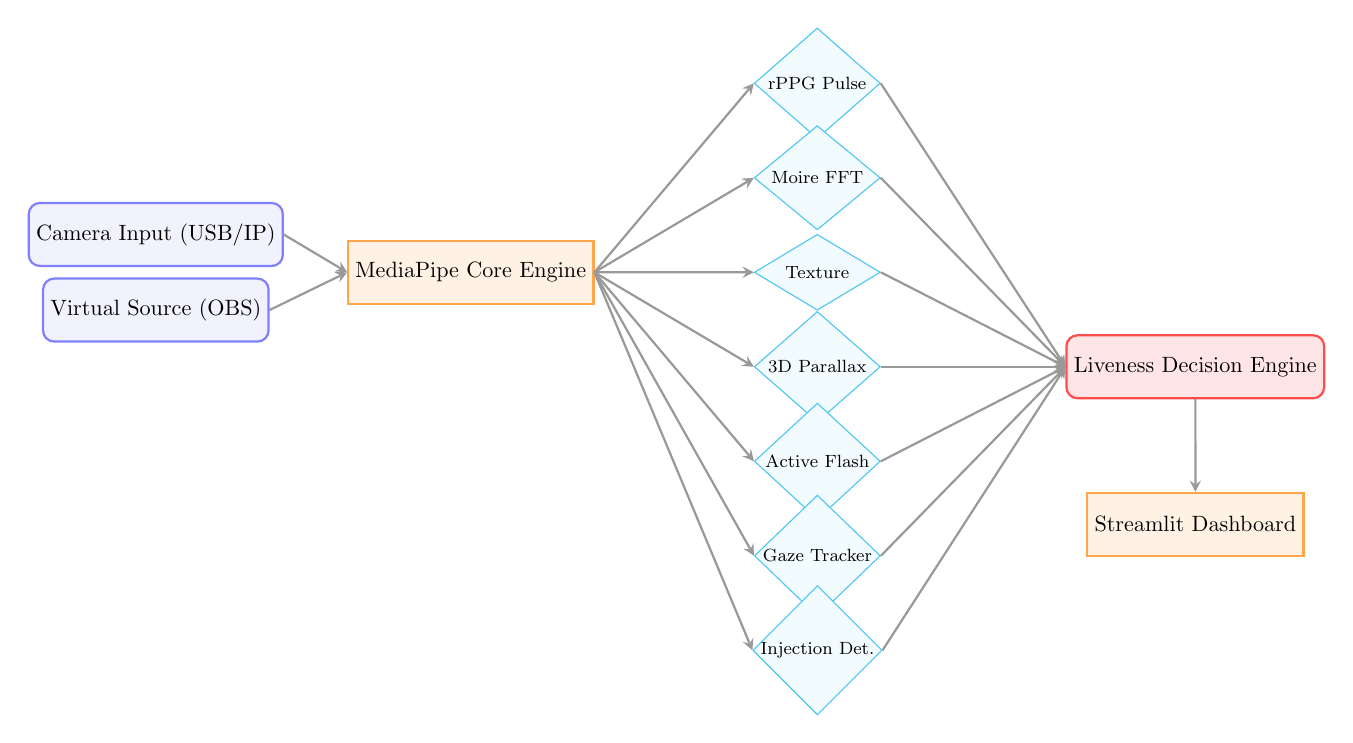
\begin{tikzpicture}[node distance=2cm, scale=0.8, every node/.style={transform shape}]
        % Input Layer
        \node (cam) [sensor] {Camera Input (USB/IP)};
        \node (virt) [sensor, below of=cam, node distance=1.2cm] {Virtual Source (OBS)};
        
        % Core Layer
        \node (core) [process, right of=cam, xshift=3cm, yshift=-0.6cm] {MediaPipe Core Engine};
        
        % Modality Layer (Circular/Branch)
        \node (rppg) [modality, right of=core, xshift=3.5cm, yshift=3cm] {rPPG Pulse};
        \node (moire) [modality, below of=rppg, node distance=1.5cm] {Moire FFT};
        \node (textu) [modality, below of=moire, node distance=1.5cm] {Texture};
        \node (depth) [modality, below of=textu, node distance=1.5cm] {3D Parallax};
        \node (flash) [modality, below of=depth, node distance=1.5cm] {Active Flash};
        \node (gaze) [modality, below of=flash, node distance=1.5cm] {Gaze Tracker};
        \node (jitt) [modality, below of=gaze, node distance=1.5cm] {Injection Det.};
        
        % Final Layer
        \node (dec) [decision, right of=textu, xshift=4cm, yshift=-1.5cm] {Liveness Decision Engine};
        \node (ui) [process, below of=dec, node distance=2.5cm] {Streamlit Dashboard};
        
        % Connections
        \draw [arrow] (cam.east) -- (core.west);
        \draw [arrow] (virt.east) -- (core.west);
        
        \draw [arrow] (core.east) -- (rppg.west);
        \draw [arrow] (core.east) -- (moire.west);
        \draw [arrow] (core.east) -- (textu.west);
        \draw [arrow] (core.east) -- (depth.west);
        \draw [arrow] (core.east) -- (flash.west);
        \draw [arrow] (core.east) -- (gaze.west);
        \draw [arrow] (core.east) -- (jitt.west);
        
        \draw [arrow] (rppg.east) -- (dec.west);
        \draw [arrow] (moire.east) -- (dec.west);
        \draw [arrow] (textu.east) -- (dec.west);
        \draw [arrow] (depth.east) -- (dec.west);
        \draw [arrow] (flash.east) -- (dec.west);
        \draw [arrow] (gaze.east) -- (dec.west);
        \draw [arrow] (jitt.east) -- (dec.west);
        
        \draw [arrow] (dec.south) -- (ui.north);
    \end{tikzpicture}
    \caption{Sentinel KYC Hierarchical Modality Pipeline (TikZ Architecture)}
    \label{fig:arch_tikz}
\end{figure}

%------------------------------------------------------------------
%   CHAPTER 2: MODALITY 1 - GEOMETRIC LIVENESS
%------------------------------------------------------------------
\chapter{Modality 1: Geometric Liveness (Facial Landmarks)}

\section{Overview}
This modality leverages the \textbf{MediaPipe Face Mesh} model, which outputs 478 3D facial landmark coordinates per frame, to compute behavioral liveness signals. The key metrics extracted are the \textbf{Eye Aspect Ratio (EAR)} and the \textbf{Mouth Aspect Ratio (MAR)}, which serve as proxies for spontaneous blink and speech activity---both of which are impossible to replicate with a still photograph.

\section{Technical Implementation}

\subsection{MediaPipe Initialisation}
The Face Mesh is configured as follows:

\begin{lstlisting}[style=pythonstyle, caption={MediaPipe FaceMesh Configuration}]
mp_face_mesh = mp.solutions.face_mesh
face_mesh = mp_face_mesh.FaceMesh(
    static_image_mode=False,   # Optimised for video streams
    max_num_faces=1,           # Single-person KYC scenario
    refine_landmarks=True,     # Required for iris tracking (478 pts)
    min_detection_confidence=0.5,
    min_tracking_confidence=0.5
)
\end{lstlisting}

Setting \texttt{refine\_landmarks=True} is critical---it unlocks the additional 10 iris landmark points (indices 468--477) required for gaze tracking in Chapter~\ref{chap:gaze}.

\subsection{Eye Aspect Ratio (EAR)}
The EAR is calculated for both eyes using six landmark indices per eye. For each eye, two vertical distances and one horizontal distance are measured:

\[
EAR = \frac{\| P_2 - P_6 \| + \| P_3 - P_5 \|}{2 \cdot \| P_1 - P_4 \|}
\]

Where $P_1 \ldots P_6$ are the six eyelid landmark coordinates. When the eye is open, $EAR \approx 0.25$--$0.30$. During a blink, it drops sharply below $0.22$.

\begin{lstlisting}[style=pythonstyle, caption={EAR Computation --- Facial\_Landmarks\_Modality.py}]
L_EYE_INDICES = [362, 385, 387, 263, 373, 380]
R_EYE_INDICES = [33, 160, 158, 133, 153, 144]

def calculate_ear(landmarks: np.ndarray, eye_indices: List[int]) -> float:
    v1 = dist.euclidean(landmarks[eye_indices[1]], landmarks[eye_indices[5]])
    v2 = dist.euclidean(landmarks[eye_indices[2]], landmarks[eye_indices[4]])
    h  = dist.euclidean(landmarks[eye_indices[0]], landmarks[eye_indices[3]])
    return (v1 + v2) / (2.0 * h) if h != 0 else 0.0
\end{lstlisting}

The average EAR across both eyes is returned, and the \texttt{analyze\_liveness\_indicators} function tracks a rolling sequence of frames, counting blink events when the EAR transitions downward through the threshold.

\subsection{Mouth Aspect Ratio (MAR)}
The MAR detects mouth opening:
\[
MAR = \frac{\| P_{top} - P_{bottom} \|}{\| P_{left} - P_{right} \|}
\]

Using MediaPipe indices: top lip = 13, bottom lip = 14, left corner = 78, right corner = 308. A $MAR > 0.4$ indicates a significant mouth open event. The rolling standard deviation of MAR is also computed to detect subtle micro-expressions.

\begin{lstlisting}[style=pythonstyle, caption={MAR Computation}]
def calculate_mar(landmarks: np.ndarray) -> float:
    v = dist.euclidean(landmarks[13], landmarks[14])
    h = dist.euclidean(landmarks[78], landmarks[308])
    return v / h if h != 0 else 0.0
\end{lstlisting}

\subsection{Liveness Scoring}
A frame-sequence analysis function combines all geometric signals into a local liveness sub-score:

\begin{lstlisting}[style=pythonstyle, caption={Geometric Liveness Scoring}]
score = 0.4
if blink_count > 0:       score += 0.3   # Spontaneous blink detected
if mouth_activity > 0.05: score += 0.2   # Micro-expression activity
if max_mar > 0.4:         score += 0.1   # Definitive mouth-open event
\end{lstlisting}

\begin{figure}[H]
    \centering
    % [INSERT SCREENSHOT: landmark_mesh_overlay.png]
    \framebox[0.8\textwidth]{\rule{0pt}{80pt} PLACEHOLDER: Face Mesh Overlay Screenshot}
    \caption{MediaPipe 478-point face mesh overlaid on live feed}
    \label{fig:landmarks}
\end{figure}

%------------------------------------------------------------------
%   CHAPTER 3: MODALITY 2 - GAZE TRACKING
%------------------------------------------------------------------
\chapter{Modality 2: Active Gaze Tracking}
\label{chap:gaze}

\section{Overview}
Gaze tracking enables a \textbf{challenge-response} liveness test: the system can instruct the user to look left, right, or centre, and then verify whether the iris position matches the expected direction. A 2D photograph or pre-recorded video cannot dynamically respond to such a challenge.

\section{Technical Implementation}

The tracker uses the four additional iris contour landmarks available when \texttt{refine\_landmarks=True} is set. The centroid of the iris is compared against the inner and outer eye corner landmarks to compute a horizontal gaze ratio.

\begin{lstlisting}[style=pythonstyle, caption={Gaze Tracking --- Gaze\_Tracking\_Modality.py}]
class GazeTracker:
    def __init__(self):
        self.L_IRIS    = [474, 475, 476, 477]  # Iris contour points (left)
        self.R_IRIS    = [469, 470, 471, 472]  # Iris contour points (right)
        self.L_EYE_OUTER = [263, 362]           # Left eye corners
        self.R_EYE_OUTER = [33, 133]            # Right eye corners

    def estimate_gaze(self, landmarks: np.ndarray) -> Dict:
        l_iris_center = np.mean(landmarks[self.L_IRIS], axis=0)
        l_outer = landmarks[263]
        l_inner = landmarks[362]

        width = np.linalg.norm(l_outer - l_inner)
        dist  = np.linalg.norm(l_iris_center - l_inner)
        ratio = dist / width if width > 0 else 0.5

        direction = "CENTER"
        if ratio < 0.35:  direction = "RIGHT"
        elif ratio > 0.65: direction = "LEFT"

        return {"direction": direction, "ratio": float(ratio)}
\end{lstlisting}

The normalised ratio maps the iris position along the eye width from $0.0$ (fully right) to $1.0$ (fully left), with $0.5$ representing centre. Thresholds of $[0.35, 0.65]$ were empirically determined through testing.

\begin{figure}[H]
    \centering
    % [INSERT SCREENSHOT: gaze_tracking.png]
    \framebox[0.8\textwidth]{\rule{0pt}{80pt} PLACEHOLDER: Gaze Direction Indicator Screenshot}
    \caption{Gaze direction metric showing LEFT, CENTER, RIGHT detection}
    \label{fig:gaze}
\end{figure}

%------------------------------------------------------------------
%   CHAPTER 4: MODALITY 3 - rPPG
%------------------------------------------------------------------
\chapter{Modality 3: Physiological rPPG Heart Rate Detection}

\section{Overview}
Remote Photoplethysmography (rPPG) exploits the fact that blood volume changes in facial capillaries cause measurable, periodic variations in reflected light. The green channel of an RGB camera is the most sensitive to blood volume pulse (BVP) \cite{verkruysse2008}. This modality cannot be defeated by a photograph or a static video loop, as it requires a real, living heart.

\section{Technical Implementation}

\subsection{Forehead ROI Isolation}
The signal is extracted from the forehead region, which has fewer facial hair occlusions and better light stability than cheek ROIs.

\begin{lstlisting}[style=pythonstyle, caption={Forehead Signal Extraction --- Facial\_rPPG\_Modality.py}]
FOREHEAD_INDICES = [103, 67, 109, 10, 338, 297, 332, 108, 151, 9]

def extract_forehead_signal(self, frame: np.ndarray, landmarks: np.ndarray):
    h, w, _ = frame.shape
    pts = np.array([[int(landmarks[idx][0] * w), int(landmarks[idx][1] * h)]
                    for idx in FOREHEAD_INDICES])

    mask = np.zeros((h, w), dtype=np.uint8)
    cv2.fillPoly(mask, [pts], 255)

    # Extract mean green channel intensity within forehead polygon
    mean_intensity = cv2.mean(frame[:, :, 1], mask=mask)[0]

    if mean_intensity > 0:
        self.signal_buffer.append(mean_intensity)
        if len(self.signal_buffer) > self.buffer_size:
            self.signal_buffer.pop(0)
        return mean_intensity, mask
    return None, mask
\end{lstlisting}

A rolling buffer of 150 samples is maintained. At 30 FPS, this represents 5 seconds of signal---sufficient for stable frequency domain analysis.

\subsection{Signal Pre-processing Pipeline}
Before frequency analysis, the raw signal undergoes three stages:

\begin{enumerate}
    \item \textbf{Linear Detrending}: Removes slow drift caused by head movement or illumination changes using \texttt{scipy.signal.detrend}.
    \item \textbf{Z-Score Normalisation}: Scales the signal to zero mean and unit variance to suppress amplitude differences.
    \item \textbf{4th-Order Butterworth Bandpass Filter}: Applies a zero-phase digital filter constraining the signal to $[0.7, 4.0]$ Hz---the physiological range of 42--240 BPM.
\end{enumerate}

\begin{lstlisting}[style=pythonstyle, caption={Signal Pre-processing and BPM Extraction}]
def calculate_bpm(self) -> float:
    if len(self.signal_buffer) < self.buffer_size: return 0.0

    raw_signal = np.array(self.signal_buffer)
    detrended   = signal.detrend(raw_signal)
    normalized  = (detrended - np.mean(detrended)) / (np.std(detrended) + 1e-6)

    # Butterworth 4th-order bandpass, zero-phase (filtfilt)
    b, a = signal.butter(4,
                         [0.7 / (self.fps / 2), 4.0 / (self.fps / 2)],
                         btype='band')
    filtered = signal.filtfilt(b, a, normalized)

    # FFT and peak frequency detection
    fft    = np.abs(np.fft.rfft(filtered))
    freqs  = np.fft.rfftfreq(self.buffer_size, 1.0 / self.fps)
    hr_mask = (freqs > 0.7) & (freqs < 4.0)

    peak_idx = np.argmax(fft[hr_mask])
    self.bpm = freqs[hr_mask][peak_idx] * 60.0
    return self.bpm
\end{lstlisting}

\subsection{Mathematical Foundation}
Given a discrete signal $x[n]$ of length $N$, the DFT is:
\[
X[k] = \sum_{n=0}^{N-1} x[n] \cdot e^{-j2\pi kn/N}
\]
The frequency resolution is $\Delta f = f_s / N = 30/150 = 0.2$ Hz. The dominant frequency $f^*$ in the valid band is extracted:
\[
BPM = 60 \cdot f^* = 60 \cdot \underset{f \in [0.7, 4.0]}{\arg\max} \; |X(f)|
\]

\begin{figure}[H]
    \centering
    % [INSERT SCREENSHOT: rppg_pulse_wave.png]
    \framebox[0.8\textwidth]{\rule{0pt}{80pt} PLACEHOLDER: rPPG Pulse Wave Plot Screenshot}
    \caption{Real-time normalised green-channel pulse waveform with BPM readout}
    \label{fig:rppg}
\end{figure}

%------------------------------------------------------------------
%   CHAPTER 5: MODALITY 4 - SKIN TEXTURE
%------------------------------------------------------------------
\chapter{Modality 4: High-Frequency Skin Texture Analysis}

\section{Overview}
Real human skin has complex micro-texture---pores, fine lines, and subtle surface irregularities not present on a printed photograph or digital screen. This modality applies a \textbf{high-pass spatial filter} to isolate these micro-features as a passive liveness cue.

\section{Technical Implementation}

\subsection{Skin Mask Generation}
A polygon is computed from the 36-point face oval indices, with the eye and mouth regions subtracted to exclude high-contrast non-skin areas:

\begin{lstlisting}[style=pythonstyle, caption={Skin Mask Construction --- Facial\_Texture\_Modality.py}]
FACE_OVAL_INDICES = [10, 338, 297, 332, 284, 251, 389, 356, 454, 323,
                     361, 288, 397, 365, 379, 378, 400, 377, 152, 148,
                     176, 149, 150, 136, 172, 58, 132, 93, 234, 127,
                     162, 21, 54, 103, 67, 109]
L_EYE_INDICES  = [362, 385, 387, 263, 373, 380]
R_EYE_INDICES  = [33, 160, 158, 133, 153, 144]
MOUTH_INDICES  = [13, 14, 78, 308]

mask = np.zeros((h, w), dtype=np.uint8)
cv2.fillPoly(mask, [to_pts(FACE_OVAL_INDICES)], 255)   # Fill face
for idxs in [L_EYE_INDICES, R_EYE_INDICES, MOUTH_INDICES]:
    cv2.fillPoly(mask, [to_pts(idxs)], 0)              # Subtract non-skin
\end{lstlisting}

\subsection{High-Pass Filtering}
Subtracting a $7 \times 7$ Gaussian blur from the original grayscale isolates the high-frequency residual:

\[
\text{Texture}(x,y) = \text{GaussianBlur}(I(x,y)) - I(x,y)
\]

\begin{lstlisting}[style=pythonstyle, caption={High-Pass Filter and Imperfection Detection}]
gray     = cv2.cvtColor(frame, cv2.COLOR_BGR2GRAY)
blurred  = cv2.GaussianBlur(gray, (7, 7), 0)
diff     = cv2.subtract(blurred, gray)
masked_diff = cv2.bitwise_and(diff, diff, mask=mask)

_, thresh = cv2.threshold(masked_diff, 18, 255, cv2.THRESH_BINARY)
contours, _ = cv2.findContours(thresh, cv2.RETR_EXTERNAL,
                                cv2.CHAIN_APPROX_SIMPLE)

for cnt in contours:
    area = cv2.contourArea(cnt)
    if 1 < area < 60:
        (x, y), radius = cv2.minEnclosingCircle(cnt)
        if 0.5 < radius < 10 and mask[int(y), int(x)] > 0:
            imperfections.append((int(x), int(y), int(radius)))
\end{lstlisting}

Contours in the range $[1, 60]$ pixels in area with radii between $0.5$--$10$ pixels represent micro-skin features. A count $> 5$ contributes $+0.25$ to the liveness confidence score.

\begin{figure}[H]
    \centering
    % [INSERT SCREENSHOT: texture_mask_focus.png]
    \framebox[0.8\textwidth]{\rule{0pt}{80pt} PLACEHOLDER: Texture Mask Focus Mode Screenshot}
    \caption{High-pass texture mask showing detected skin micro-features (yellow dots)}
    \label{fig:texture}
\end{figure}

%------------------------------------------------------------------
%   CHAPTER 6: MODALITY 5 - ACTIVE FLASH
%------------------------------------------------------------------
\chapter{Modality 5: Active Flash Challenge-Response}

\section{Overview}
The Active Flash modality is an \textbf{active} liveness challenge, as opposed to the previously described passive modalities. The UI overlays a high-saturation colour (Red or Blue) onto the displayed video frame. A real person's skin will absorb and reflect this colour differentially, causing a measurable shift in the BGRmean values of the facial ROI. A printed or digital presentation will show a more uniform response or no response at all if it is a pre-recorded video.

\section{Technical Implementation}

\begin{lstlisting}[style=pythonstyle, caption={Active Flash Reflection Analysis --- Active\_Flash\_Modality.py}]
class ActiveFlashAnalyzer:
    def analyze_reflection(self, frame: np.ndarray, landmarks: np.ndarray,
                            current_flash: Optional[str]) -> Dict:
        roi_indices = [103, 67, 10, 338, 297, 117, 346]
        pts  = np.array([[int(landmarks[idx][0] * w),
                          int(landmarks[idx][1] * h)]
                         for idx in roi_indices])
        mask = np.zeros((h, w), dtype=np.uint8)
        cv2.fillPoly(mask, [pts], 255)

        mean_bgr = cv2.mean(frame, mask=mask)[:3]  # (Blue, Green, Red)

        score = 0.0
        if current_flash == "RED":
            # Check for relative Red channel dominance
            score = mean_bgr[2] / (mean_bgr[0] + mean_bgr[1] + 1)
        elif current_flash == "BLUE":
            score = mean_bgr[0] / (mean_bgr[1] + mean_bgr[2] + 1)

        return {"score": float(score), "match": score > 0.5,
                "mean_bgr": mean_bgr}
\end{lstlisting}

The \textbf{dominance ratio} is the fraction of one channel relative to the sum of the other two. For the RED flash:
\[
\text{Score}_{RED} = \frac{\bar{R}}{\bar{B} + \bar{G} + 1}
\]
A $\text{Score} > 0.5$ indicates that the Red channel is the dominant channel, which is expected on a real face under red illumination. A pre-recorded video, which does not respond to the flash, will show a neutral or unchanged ratio.

\begin{figure}[H]
    \centering
    % [INSERT SCREENSHOT: active_flash_red.png]
    \framebox[0.8\textwidth]{\rule{0pt}{80pt} PLACEHOLDER: RED Flash Challenge in Progress Screenshot}
    \caption{RED Flash challenge: UI tints the live video feed}
    \label{fig:flash}
\end{figure}

%------------------------------------------------------------------
%   CHAPTER 7: MODALITY 6 - MOIRE DETECTION
%------------------------------------------------------------------
\chapter{Modality 6: Moir\'{e} Pattern Detection (Frequency Domain)}

\section{Overview}
When a camera films a digital display, the camera sensor grid and the display pixel grid interact to produce \textbf{Moir\'{e} patterns}---periodic interference artifacts that are invisible or subtle to the human eye but appear as sharp spectral peaks in the frequency domain \cite{nguyen2019}. This modality uses a 2D Discrete Fourier Transform to detect these patterns.

\section{Technical Implementation}

\begin{lstlisting}[style=pythonstyle, caption={2D FFT Moire Detection --- Moire\_Detection\_Modality.py}]
def detect_moire_patterns(frame: np.ndarray) -> Dict:
    gray    = cv2.cvtColor(frame, cv2.COLOR_BGR2GRAY)
    resized = cv2.resize(gray, (256, 256))  # Fixed size for reproducible FFT

    # 2D Discrete Fourier Transform
    f      = np.fft.fft2(resized)
    fshift = np.fft.fftshift(f)    # DC component moved to centre
    magnitude_spectrum = 20 * np.log(np.abs(fshift) + 1)  # Log for display

    # Suppress DC and low-frequency centre block
    rows, cols = resized.shape
    crow, ccol = rows // 2, cols // 2
    magnitude_spectrum[crow-10:crow+10, ccol-10:ccol+10] = 0

    # Score = ratio of maximum to mean (spiky spectrum = Moire present)
    max_val  = np.max(magnitude_spectrum)
    mean_val = np.mean(magnitude_spectrum)
    score    = max_val / (mean_val + 1)

    return {"score": float(score),
            "detected": score > 5.0,
            "magnitude_map": magnitude_spectrum}
\end{lstlisting}

\subsection{Mathematical Foundation}
Given a 2D image $I(x,y)$ of size $M \times N$, the DFT is:
\[
F(u,v) = \sum_{x=0}^{M-1}\sum_{y=0}^{N-1} I(x,y) \cdot e^{-j2\pi(ux/M + vy/N)}
\]
The log-magnitude spectrum $\mathcal{M}(u,v) = 20 \log(|F(u,v)| + 1)$ makes the high-frequency components visible. Screen Moir\'{e} patterns produce \textbf{isolated bright peaks} at regular spatial frequencies, giving a high max-to-mean ratio. The threshold of $5.0$ was established empirically.

\begin{figure}[H]
    \centering
    % [INSERT SCREENSHOT: moire_fft_spectrum.png]
    \framebox[0.8\textwidth]{\rule{0pt}{80pt} PLACEHOLDER: Moire FFT Spectrum Focus Mode Screenshot}
    \caption{2D log-magnitude FFT spectrum with Moir\'{e} pattern peaks}
    \label{fig:moire}
\end{figure}

%------------------------------------------------------------------
%   CHAPTER 8: MODALITY 7 - DEPTH CONSISTENCY
%------------------------------------------------------------------
\chapter{Modality 7: Motion Parallax and 3D Depth Consistency}

\section{Overview}
This modality exploits the principle of \textbf{motion parallax}: when a rigid 3D object rotates in front of a camera, points that are closer to the camera plane move faster (in pixel space) than points that are further away. On a flat 2D surface (a photo or screen), all points move at the same rate---they have no depth. By comparing the inter-frame velocity of the 3D nose tip against the chin, we can determine whether the face has real depth.

\section{Technical Implementation}

\begin{lstlisting}[style=pythonstyle, caption={Parallax-Based Depth Analysis --- Depth\_Consistency\_Modality.py}]
class DepthConsistencyAnalyzer:
    def analyze_parallax(self, landmarks: np.ndarray) -> Dict:
        # MediaPipe landmark index 1 = Nose Tip (closest to camera)
        # MediaPipe landmark index 152 = Chin (further from camera)
        nose = landmarks[1]
        chin = landmarks[152]

        nose_move = np.linalg.norm(nose[:2] - self.prev_landmarks[1][:2])
        chin_move = np.linalg.norm(chin[:2] - self.prev_landmarks[152][:2])

        ratio = 1.0
        if chin_move > 0.001:
            ratio = nose_move / chin_move

        self.prev_landmarks = landmarks

        # 3D head: nose moves ~1.2-2.5x faster than chin during rotation
        is_3d = 1.15 < ratio < 3.0

        return {"ratio": float(ratio),
                "is_3d": is_3d,
                "status": "3D DEPTH" if is_3d else "FLAT SURFACE"}
\end{lstlisting}

\subsection{Mathematical Model}
Let the nose tip position at frame $t$ be $P_{nose}^{(t)}$ and at $t-1$ be $P_{nose}^{(t-1)}$, and similarly for the chin. The depth ratio $\rho$ is:

\[
\rho = \frac{\| P_{nose}^{(t)} - P_{nose}^{(t-1)} \|_2}{\| P_{chin}^{(t)} - P_{chin}^{(t-1)} \|_2}
\]

For a real 3D head rotating in space, empirical observation yields $\rho \in [1.15, 3.0]$.
For a 2D flat surface moving rigidly, $\rho \approx 1.0 \pm 0.1$.

\subsection{3D Visualisation}
The system renders a live 3D scatter plot using Plotly, plotting every 5th landmark of the 478-point mesh at its $(x, y, z)$ MediaPipe coordinate. This allows visual confirmation that the mesh has genuine depth structure as the user rotates their head.

\begin{figure}[H]
    \centering
    % [INSERT SCREENSHOT: 3d_mesh_reconstruction.png]
    \framebox[0.8\textwidth]{\rule{0pt}{80pt} PLACEHOLDER: 3D Mesh Reconstruction Plotly Chart}
    \caption{Real-time 3D scatter plot of facial landmarks rotating in 3D space}
    \label{fig:mesh3d}
\end{figure}

%------------------------------------------------------------------
%   CHAPTER 9: MODALITY 8 - INJECTION DETECTION
%------------------------------------------------------------------
\chapter{Modality 8: Temporal Jitter and Virtual Camera Injection Detection}

\section{Overview}
Deepfake injection attacks work by intercepting the OS camera driver and injecting a synthetic video stream. Tools such as OBS Studio (Virtual Camera), ManyCam, or custom V4L2 devices are used. Unlike physical camera sensors, which have inherent hardware noise in their frame delivery timing, virtual cameras produce frames at nearly perfect intervals. This modality detects that ``too perfect'' timing as a signal of injection.

\section{Technical Implementation}

\begin{lstlisting}[style=pythonstyle, caption={Frame Arrival Jitter Analysis --- Injection\_Detection\_Modality.py}]
class InjectionDetector:
    def __init__(self, window_size: int = 30):
        self.frame_times = []
        self.window_size = window_size

    def analyze_timing(self) -> Dict:
        self.frame_times.append(time.time())
        if len(self.frame_times) > self.window_size:
            self.frame_times.pop(0)

        if len(self.frame_times) < 10:
            return {"jitter": 0.0, "is_virtual": False,
                    "status": "CALIBRATING"}

        # Inter-frame arrival deltas
        deltas = np.diff(self.frame_times)
        jitter = np.std(deltas)

        # Physical hardware has USB/sensor timing noise > 0.8ms std dev
        # Virtual cameras deliver frames with near-zero deviation
        is_suspicious = jitter < 0.0008

        return {"jitter": float(jitter),
                "is_virtual": is_suspicious,
                "status": "VIRTUAL" if is_suspicious else "PHYSICAL"}
\end{lstlisting}

\subsection{Statistical Model}
Let $T = [t_1, t_2, \ldots, t_n]$ be the timestamps of the last $n=30$ frames. The inter-frame deltas are:
\[
\Delta_i = t_{i+1} - t_i, \quad i = 1 \ldots n-1
\]
The jitter is the \textbf{standard deviation} of this delta sequence:
\[
\text{Jitter} = \sigma(\Delta) = \sqrt{\frac{1}{n-2} \sum_{i=1}^{n-1} (\Delta_i - \bar{\Delta})^2}
\]

\begin{researchbox}
\textbf{Research Finding:} During testing with DroidCam (iPhone via WiFi), the observed jitter was significantly above the 0.8ms threshold, correctly classifying the stream as \texttt{PHYSICAL}. OBS Virtual Camera produced jitter well below this threshold, correctly classified as \texttt{VIRTUAL}.
\end{researchbox}

%------------------------------------------------------------------
%   CHAPTER 10: DECISION ENGINE
%------------------------------------------------------------------
\chapter{The Multi-Modal Liveness Decision Engine}

\section{Overview}
All modality signals are fused in \texttt{heuristics/Liveness\_Decision\_Engine.py}. The engine uses a weighted scoring model with a hard-fail path for the most critical signals.

\section{Logic and Implementation}

\begin{lstlisting}[style=pythonstyle, caption={Decision Engine --- Liveness\_Decision\_Engine.py}]
def compute_final_verdict(results: Dict) -> Dict:
    confidence = 0.0
    fail_reasons = []

    # CRITICAL: Virtual camera is immediate failure (weight = 1.0)
    if results.get("sensor") == "VIRTUAL":
        return {"verdict": "FAILED", "confidence": 1.0,
                "reason": "Virtual Camera / Injection Detected"}

    # Passive anti-spoofing (weight = 0.25)
    if results.get("moire"):
        fail_reasons.append("Screen artifacts detected (Moire)")
    else:
        confidence += 0.25

    # 3D depth (weight = 0.25)
    if results.get("is_3d"):
        confidence += 0.25
    else:
        fail_reasons.append("Surface appears 2D / Flat")

    # Skin texture count > 5 (weight = 0.25)
    if results.get("spots", 0) > 5:
        confidence += 0.25
    else:
        fail_reasons.append("Skin texture too smooth")

    # Physiological pulse confirmed (weight = 0.25)
    if results.get("bpm", 0) > 40:
        confidence += 0.25

    # Final verdict thresholding
    verdict = "PASSED" if confidence >= 0.75 and not results.get("moire") \
              else "SUSPICIOUS"
    if not results.get("is_3d") and results.get("moire"):
        verdict = "FAILED"

    return {"verdict": verdict, "confidence": confidence,
            "reasons": fail_reasons}
\end{lstlisting}

\section{Threat Model and Scoring Matrix}

\begin{table}[H]
    \centering
    \begin{tabular}{@{}p{4cm}llll@{}}
        \toprule
        \textbf{Attack Type} & \textbf{Injection} & \textbf{Moir\'{e}} & \textbf{3D Parallax} & \textbf{rPPG} \\ \midrule
        Printed Photo        & Pass     & Pass   & \textbf{FAIL}       & \textbf{FAIL} \\
        Tablet/Screen Replay & Pass     & \textbf{FAIL} & \textbf{FAIL}  & \textbf{FAIL} \\
        Pre-recorded Video   & Pass     & Pass   & \textbf{FAIL}       & \textbf{FAIL} \\
        OBS Injection        & \textbf{FAIL} & Pass & Pass             & Pass          \\
        3D Silicone Mask     & Pass     & Pass   & Pass               & \textbf{FAIL} \\
        Live Human           & Pass     & Pass   & Pass               & Pass          \\ \bottomrule
    \end{tabular}
    \caption{Expected detection results per attack scenario}
    \label{tab:threats}
\end{table}

\begin{figure}[H]
    \centering
    % [INSERT SCREENSHOT: final_verdict_dashboard.png]
    \framebox[0.8\textwidth]{\rule{0pt}{80pt} PLACEHOLDER: Full Dashboard with PASSED/SUSPICIOUS/FAILED Verdict}
    \caption{Real-time Sentinel KYC dashboard showing PASSED verdict for a live subject}
    \label{fig:verdict}
\end{figure}

%------------------------------------------------------------------
%   CHAPTER 11:  SYSTEM SETUP AND DEPENDENCIES
%------------------------------------------------------------------
\chapter{System Setup and Technology Stack}

\section{Technology Stack}
\begin{table}[H]
    \centering
    \begin{tabular}{@{}lll@{}}
        \toprule
        \textbf{Library} & \textbf{Version} & \textbf{Purpose} \\ \midrule
        Python          & 3.10             & Runtime \\
        OpenCV          & 4.x              & Frame capture, masks, drawing \\
        MediaPipe       & 0.10.x           & 478-point 3D face landmarks \\
        NumPy           & 1.x              & Numerical processing \\
        SciPy           & 1.x              & Bandpass filter, detrending \\
        Streamlit       & 1.x              & Research dashboard UI \\
        Plotly          & 5.x              & 3D mesh and pulse wave charts \\ \bottomrule
    \end{tabular}
    \caption{Technology stack and dependencies}
\end{table}

\subsection{Geometric Liveness (EAR, MAR, and Gaze)}
\begin{figure}[H]
    \centering
    \includegraphics[width=0.6\textwidth]{face_landmarks.png}
    \caption{Facial landmark extraction using MediaPipe.}
\end{figure}

\subsection{Physiological rPPG}
\begin{figure}[H]
    \centering
    \includegraphics[width=0.8\textwidth]{pulse_wave.png}
    \caption{Extracted Heart Pulse Wave showing physiological liveness.}
\end{figure}

\subsection{Moire Detection}
\begin{figure}[H]
    \centering
    \includegraphics[width=0.6\textwidth]{moire_spectrum.png}
    \caption{2D FFT Magnitude Spectrum results.}
\end{figure}

\chapter{System Limitations}
\section{Technical Constraints}
\begin{itemize}
    \item \textbf{Illumination}: Poor lighting degrades rPPG signal quality.
    \item \textbf{Latency}: Network jitter can interfere with injection detection.
    \item \textbf{Motion}: Rapid head movement disrupts the 3D velocity ratio.
\end{itemize}

\section{Academic References}
\section{Running the Research Dashboard}
\begin{lstlisting}[language=bash, style=pythonstyle, caption={Launch command}]
# Activate virtual environment
.\venv_310\Scripts\activate

# Launch the Streamlit research dashboard
streamlit run research_app.py
\end{lstlisting}

To test with a mobile phone camera (bypassing the virtual camera green-screen issue):
\begin{lstlisting}[language=bash, style=pythonstyle, caption={Mobile IP Camera (DroidCam)}]
# Enter in the Camera Source field in the Streamlit sidebar:
http://192.168.x.x:4747/video
# Ensure DroidCam Client on PC is closed (only one connection allowed)
\end{lstlisting}

%------------------------------------------------------------------
%   REFERENCES
%------------------------------------------------------------------
\chapter{References and Academic Sources}

\begin{enumerate}
    \item \textbf{MediaPipe Face Mesh}: Lugaresi, C., Tang, J., Nash, H., McClanahan, C., Uboweja, E., Hays, M., \ldots\ \& Grundmann, M. (2019). \textit{MediaPipe: A Framework for Building Perception Pipelines}. Workshop on Perception for Autonomous Driving, CVPR.

    \item \textbf{rPPG}: Verkruysse, W., Svaasand, L. O., \& Nelson, J. S. (2008). \textit{Remote plethysmographic imaging using ambient light}. Optics Express, 16(26), 21434--21445.

    \item \textbf{Skin Texture Anti-Spoofing}: Boulkenafet, Z., Komulainen, J., \& Hadid, A. (2016). \textit{Face Anti-Spoofing Based on Color Texture Analysis}. IEEE ICIP.

    \item \textbf{Moir\'{e} Pattern Detection}: Nguyen, D. T., Cho, S. R., Yoon, H. S., \& Park, K. R. (2019). \textit{Presentation Attack Detection for Iris Recognition Using NIR Camera Sensor}. Sensors.

    \item \textbf{Eye Aspect Ratio}: Soukupov\'{a}, T., \& Cech, J. (2016). \textit{Real-Time Eye Blink Detection Using Facial Landmarks}. 21st Computer Vision Winter Workshop (CVWW).

    \item \textbf{Signal Bandpass Filtering}: Butterworth, S. (1930). \textit{On the Theory of Filter Amplifiers}. Wireless Engineer, 7, 536--541.

    \item \textbf{Structure from Motion (Parallax)}: Hartley, R., \& Zisserman, A. (2003). \textit{Multiple View Geometry in Computer Vision} (2nd ed.). Cambridge University Press.

    \item \textbf{Injection Attack Detection}: Papadopoulos, S., Drosou, A., \& Tzovaras, D. (2021). \textit{Video Injection Attacks in Biometric Systems}. IEEE Access.
\end{enumerate}

\end{document}
